\section{Performa Kecepatan Akselerator}

Terdapat dua pengujian performa kecepatan yang penting untuk diujikan yaitu performa kecepatan akselerator dalam proses pembelajaran \ac{RL} dan dalam proses \textit{inference}. Kedua proses ini digunakan di waktu yang berbeda dan memiliki signifikansi aplikasi yang berbeda juga. Selengkapnya, hasil data dan pembahasan yang didapat untuk uji performa akselerator ini akan dibahas pada sub subbab \ref{subsec:performance-learning} dan \ref{subsec:performance-inference}.

\subsection{Performa Pembelajaran \acl{RL}}
\label{subsec:performance-learning}

Untuk menguji performa pembelajaran \ac{RL} pada akselerator, dilakukan pengujian kecepatan untuk melakukan pembelajaran masalah labirin dengan besar 5 x 5. Berikut, pada gambar \ref{fig:5x5}, merupakan hasil dari hasil pengujian.

\begin{figure}[h]
	\centering
	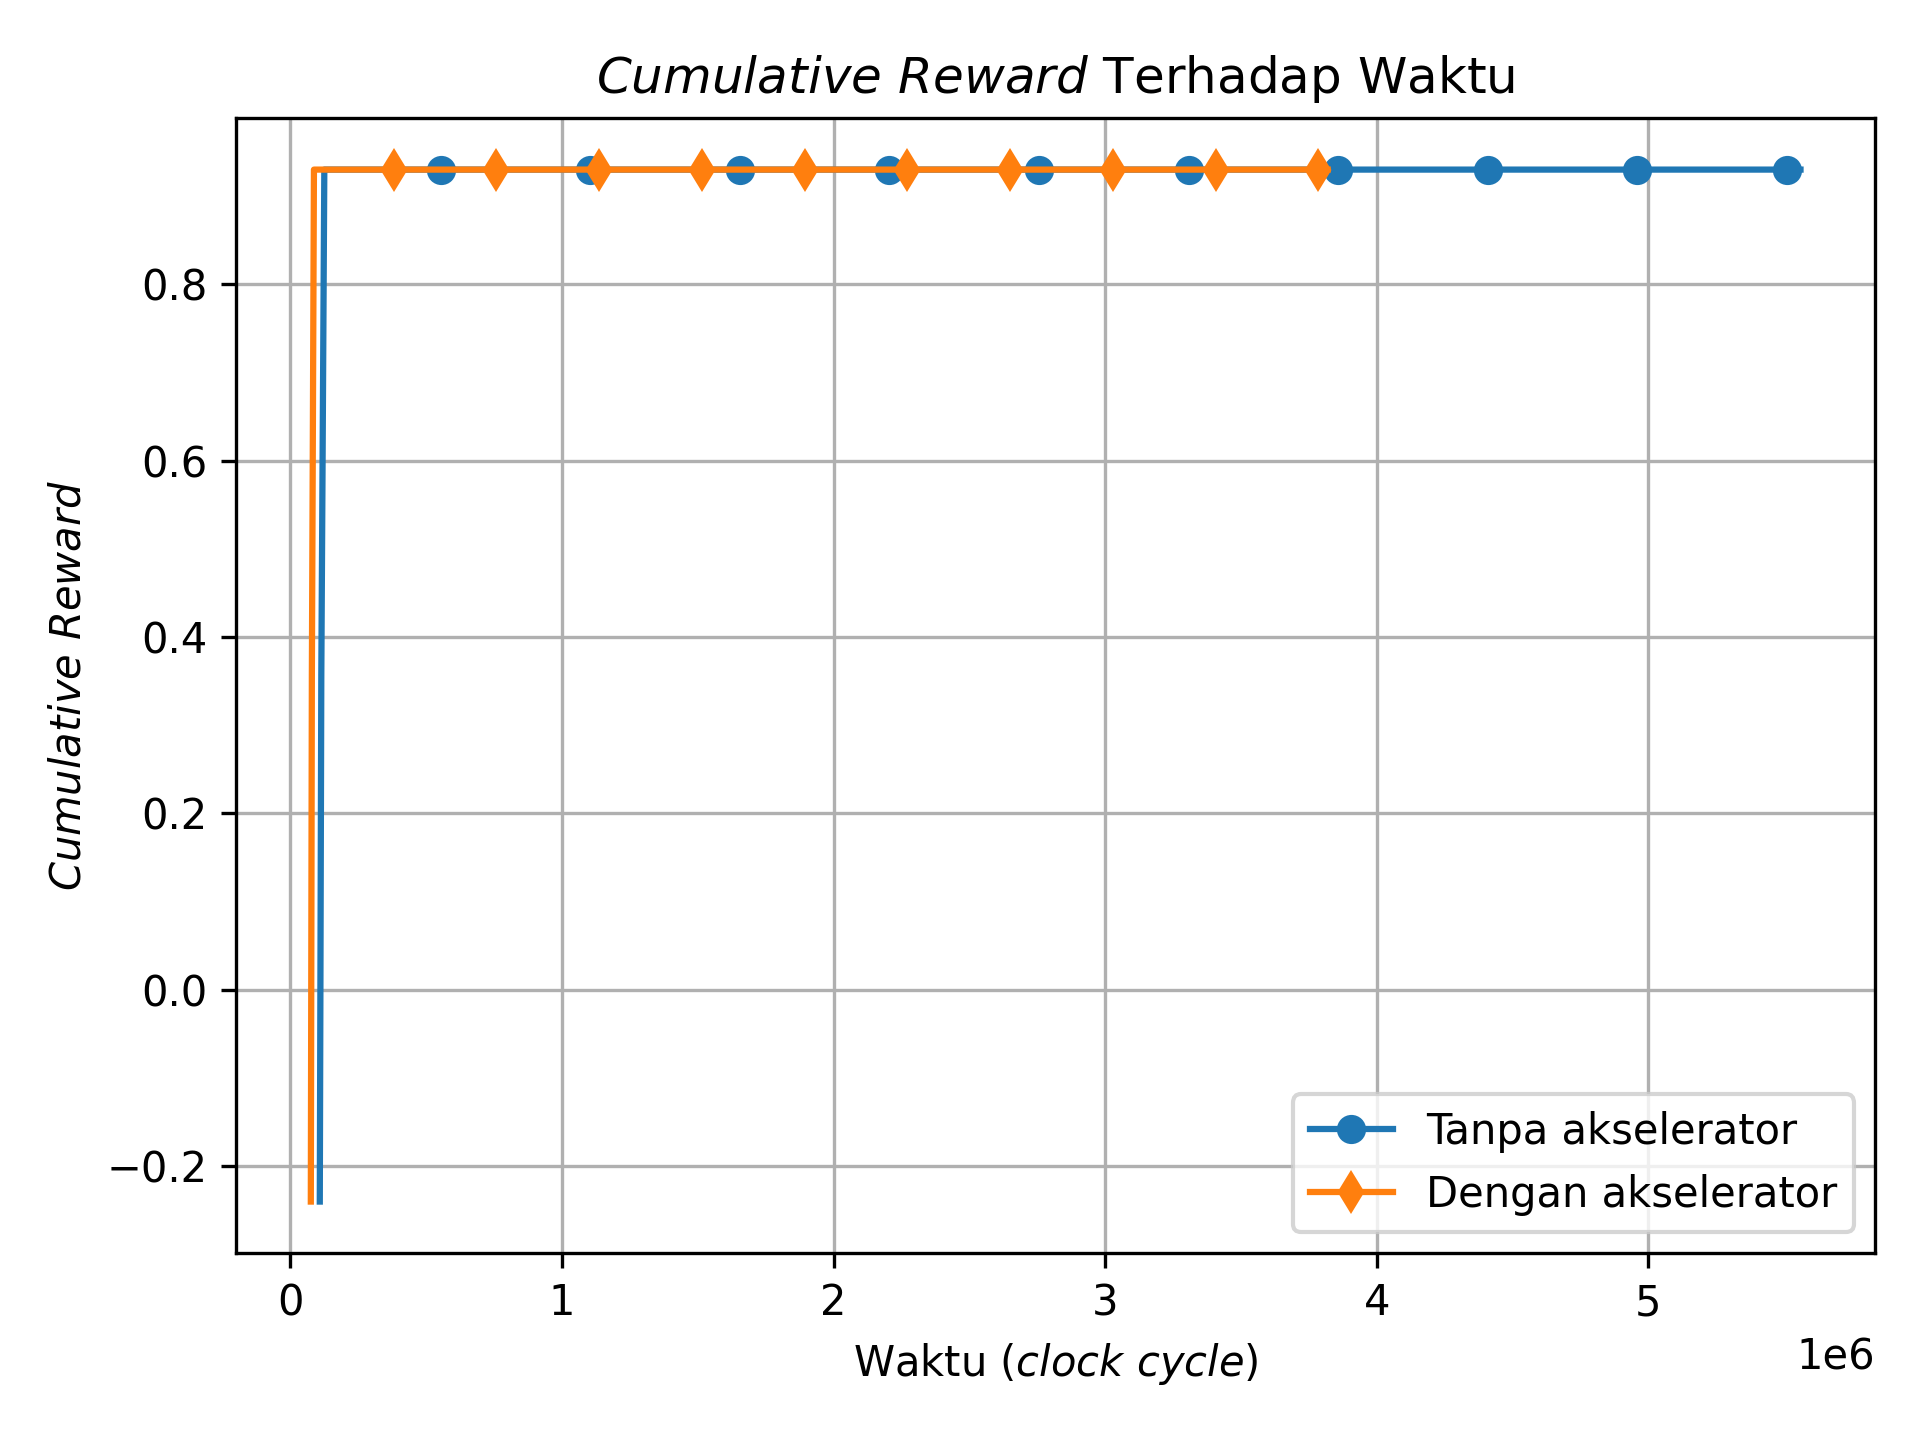
\includegraphics[width=1\textwidth]{chapter-4/5x5.png}
	\caption{Hasil pengujian akselerator terhadap perangkat lunak pada besar labirin 5 x 5}
	\label{fig:5x5}
\end{figure}

Gambar \ref{fig:5x5} merupakan plot grafik antara \textit{cumulative reward} terhadap waktu yang diperlukan untuk melakukan pembelajaran. Dapat dilihat, bahwa penggunaan akselerator mempercepat pembelajaran tanpa mengubah nilai \textit{cumulative reward} sama sekali. Pengujian pada gambar \ref{fig:5x5}, dilakukan dengan 1000 jumlah episode pembelajaran. Agar dapat melihat tren dari waktu pembelajaran terhadap episode, dibuatlah grafik yang diplot pada gambar \ref{fig:episode_vs_actime}.

\begin{figure}[htbp]
	\centering
	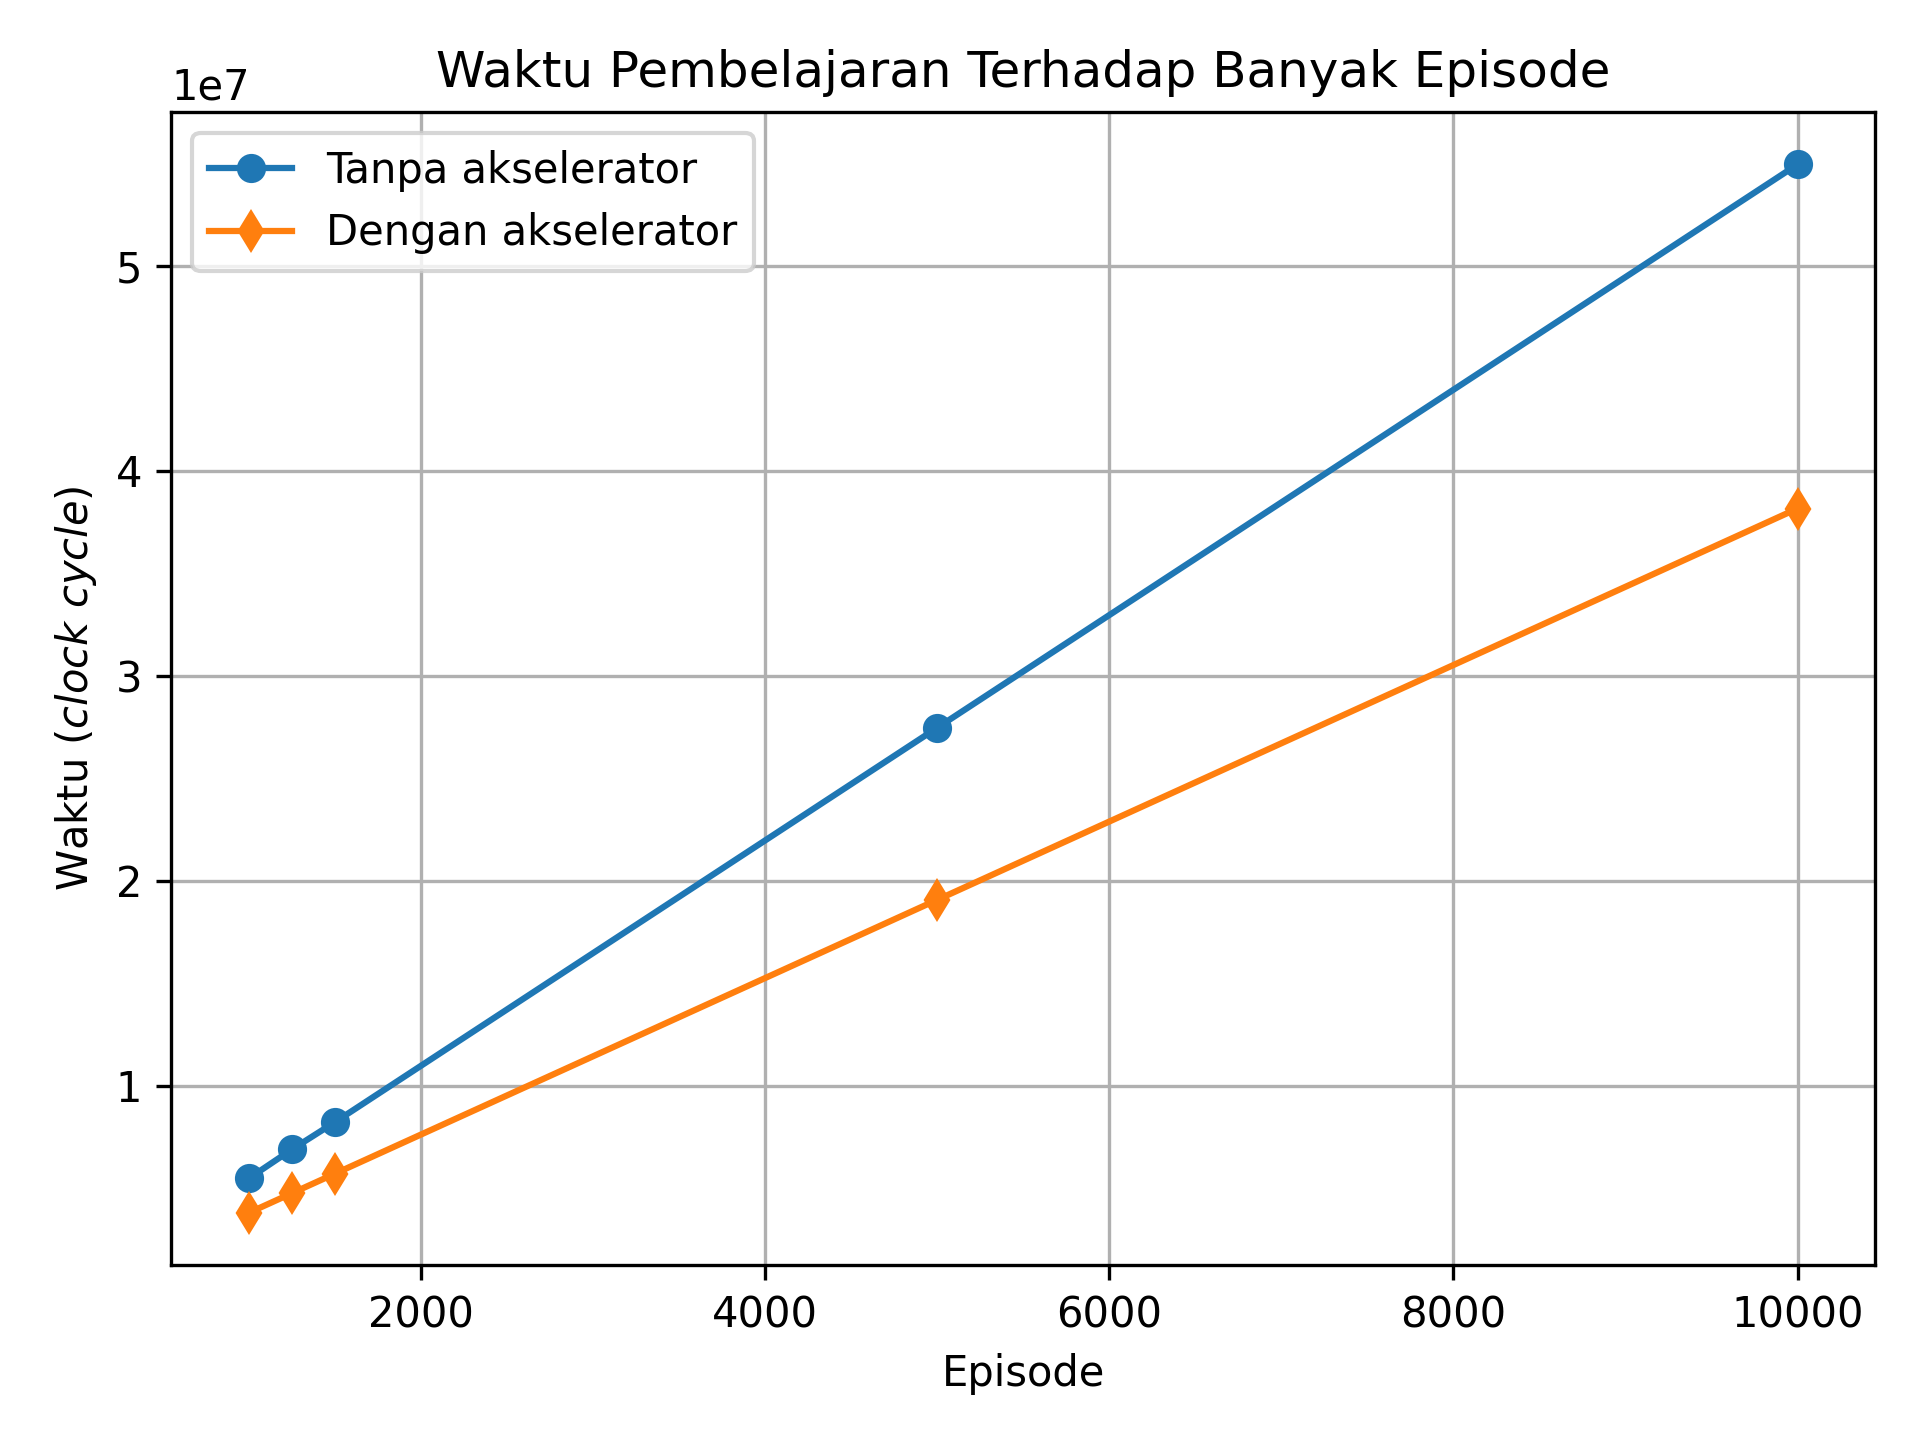
\includegraphics[width=1\textwidth]{chapter-4/episode_vs_actime.png}
	\caption{Hasil pengujian akselerator pada berbagai macam episode maksimal}
	\label{fig:episode_vs_actime}
\end{figure}

Pada gambar \ref{fig:episode_vs_actime}, diplot tren waktu yang diambil terhadap variasi episode. Kedua implementasi, baik pada perangkat lunak maupun pada akselerator perangkat keras, memiliki tren linear dalam peningkatan waktu yang diperlukan terhadap episode. Namun, implementasi perangkat keras memiliki gradien yang lebih kecil dari implementasi perangkat lunak. Setelah dilakukan regresi, didapat bahwa masing-masing garis memiliki persamaan sebagai berikut.

\begin{enumerate}
	\item Perangkat lunak: $y = 5494,05x + 7364,74$
	\item Akselerator perangkat keras: $y = 3816,97x - 4681,35$
\end{enumerate}

Dengan demikian, dapat disimpulkan bahwa meskipun kompleksitas teoritis dari perangkat lunak dan akselerator perangkat keras sama, $O(n)$, tetapi implementasi akselerator perangkat keras akan menjadi semakin efisien bila dibandingkan kepada implementasi perangkat lunak pada episode yang semakin tinggi.

\subsection{Performa \textit{Inference} \acl{RL}}
\label{subsec:performance-inference}

Pada pengujian performa akselerator untuk proses \textit{inference}, dilakukan pengukuran waktu yang diperlukan untuk melakukan metode $\epsilon$-greedy. Pada implementasi akselerator perangkat keras, digunakan instruksi q.max sedangkan pada implementasi perangkat lunak dilakukan pembandingan nilai maksimal menggunakan kondisional dan pengulangan. Berikut merupakan hasil yang didapatkan dari uji pada permasalahan labirin.

\begin{enumerate}
	\item Perangkat lunak: 393 \textit{clock cycles}
	\item Akselerator perangkat keras: 13 \textit{clock cycles}
\end{enumerate}

Kecepatan yang didapatkan dari akselerator mencapai sekitar 30,23 kali lebih cepat daripada perangkat lunak. Kecepatan ini kemudian dicoba dengan variasi $N_a$ yang dilakukan agar dapat melihat sebaik apa penggunaan akselerator pada \textit{large branching factor}. Gambar \ref{fig:speed-action} merupakan plot dari performa akselerator dengan variasi $N_a$.

\begin{figure}[htbp]
	\centering
	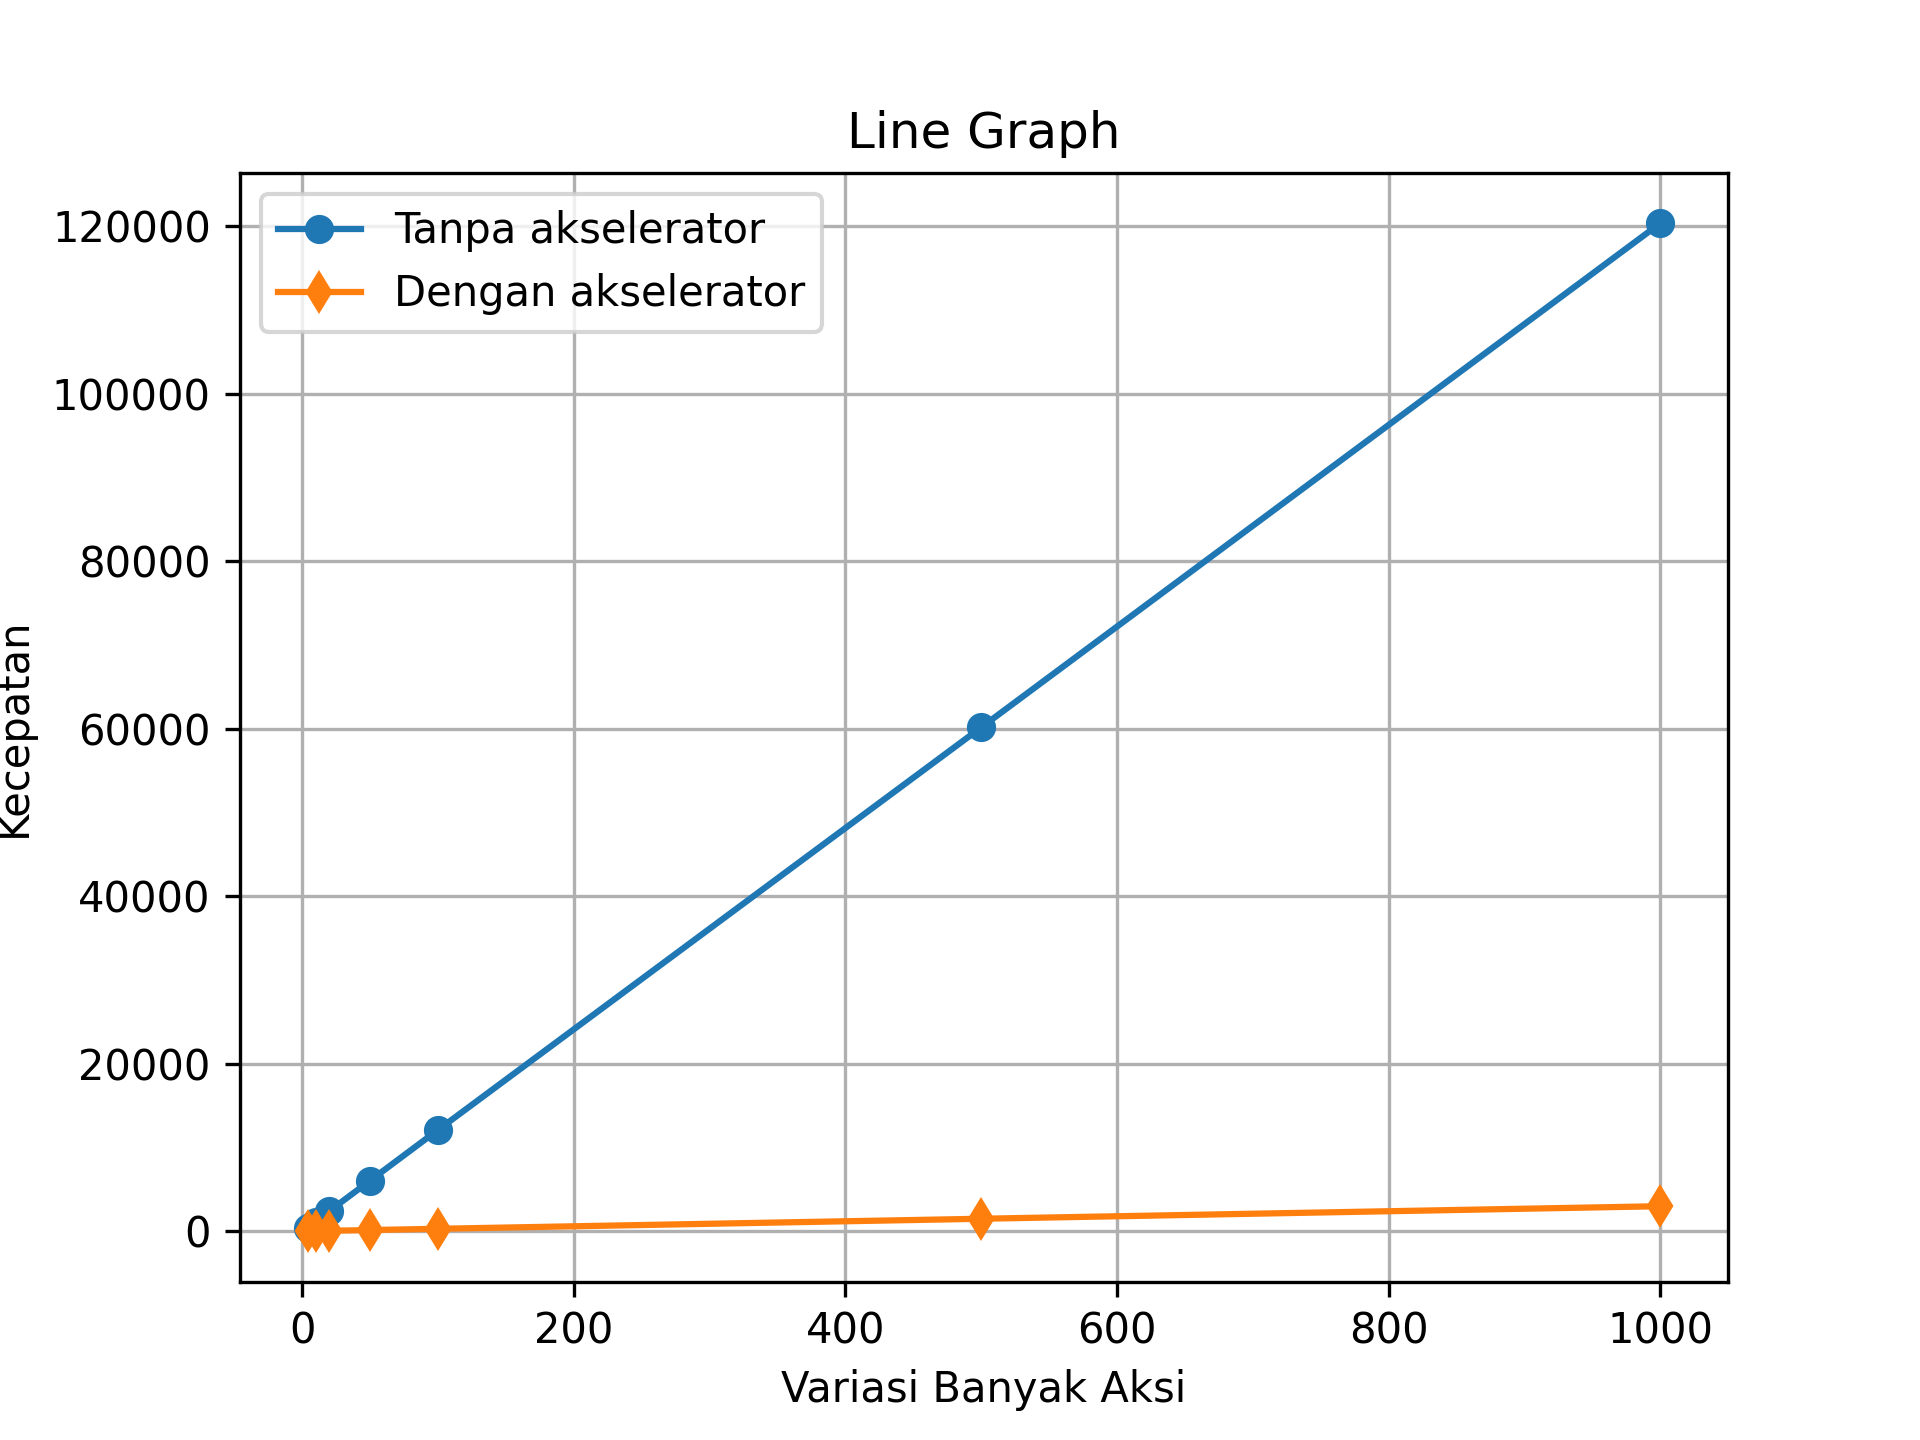
\includegraphics[width=1\textwidth]{chapter-4/plot-speed-action.png}
	\caption{Hasil pengujian kecepatan akselerator dengan variasi $N_a$}
	\label{fig:speed-action}
\end{figure}

Gambar \ref{fig:speed-action} memiliki sifat yang cukup mirip dengan gambar \ref{fig:episode_vs_actime}, yaitu sifat linear dari kedua profil kecepatan. Namun, perbedaan gradien yang dimiliki oleh \ref{fig:speed-action} jauh lebih besar lagi. Berikut merupakan detail dari masing-masing persamaan garis.

\begin{enumerate}
	\item Perangkat lunak: $y = 120,36x - 12,55$
	\item Akselerator perangkat keras: $y = 3x - 3,19$
\end{enumerate}

Apabila digunakan $N_a$ yang bernilai 1.000, maka banyaknya \textit{clock cycles} yang diperlukan untuk menyelesaikan $\epsilon$-greedy adalah 120.342 pada perangkat lunak dan 2.992 pada akselerator perangkat keras. \textit{Processor} VeeR EL2 yang digunakan pada eksperimen ini memiliki kecepatan 12,5 MHz. Sehingga waktu \textit{delay} adalah 9 milisekon untuk perangkat lunak dan 0,2 milisekon untuk akselerator perangkat lunak. Waktu \textit{delay} tersebut digunakan untuk mensimulasikan implikasi \textit{real time} pada permasalahan \textit{cart pole balancing}.

Hasil percobaan menggunakan permasalahan \textit{cart pole balancing} memperlihatkan bahwa dengan delay 9 milisekon dari perangkat lunak, \textit{cart pole} hanya bisa bertahan 4 detik sebelum akhirnya terjatuh. Sedangkan pada kasus delay 0,2 milisekon dari akselerator perangkat keras \textit{cart pole} berhasil mempertahankan posisinya setelah selama 1 menit. Analisis secara analitik pada lampiran \ref{appendix:real-time}, menunjukkan hal yang sama. Ketika ruang keadaan diskrit diberikan $T_s = 9 \text{ ms}$, hasilnya lebih tidak stabil dibanding ketika diberikan $T_s = 0,2 \text{ ms}$.
